\chapter{Weak Fields, Gravitational Waves, and the Action Principle}

We follow the lecture in the spirit in which it was given: not as a place to perform a full blackboard derivation of Einstein's equations, but as a place to see their structure, to understand why weak gravitational disturbances behave like waves, and to separate real curvature from mere coordinate ripple. These companion notes follow Leonard Susskind's presentation closely, with explicit credit to Leonard Susskind, LazyingArt LLC, and Video2Book. We will keep one sign convention fixed throughout, namely
\[
\eta_{\mu\nu}=\mathrm{diag}(-1,1,1,1),
\]
so that the spatial metric in a fixed-time slice begins with positive unit entries.

\section{Weak Fields and the Vacuum Background}

The lecture begins by lowering the computational temperature on purpose. General relativity is perfectly capable of producing pages of algebra, but that is not the point here. The point is to understand what the equations are trying to say when the gravitational field is weak, and in particular what they say about gravitational waves.

We begin in vacuum, with no energy-momentum tensor on the right-hand side. Einstein's equations then read
\begin{align}
R_{\mu\nu}-\frac12 g_{\mu\nu}R &= 0.
\end{align}
If we take the trace, then in four dimensions
\begin{align}
g^{\mu\nu}\!\left(R_{\mu\nu}-\frac12 g_{\mu\nu}R\right)=R-2R=0,
\end{align}
and therefore
\begin{align}
R=0.
\end{align}
Substituting back, the vacuum equation simplifies to
\begin{align}
R_{\mu\nu}=0.
\end{align}

\begin{figure}[t]
\centering

\includegraphics[width=0.68\textwidth]{lecture_10_figure_02.png}
\caption{The operational starting point of the lecture: the vacuum equation \(R_{\mu\nu}=0\) written almost alone on the board.}
\end{figure}

Now we ask the question Susskind asks immediately: what is an equilibrium situation? In this lecture the answer is very sharp. It is a solution with no time dependence and with no matter on the right-hand side. There is really only one such equilibrium around which to build the weak-field discussion: empty flat spacetime.

But here the lecture makes an important conceptual correction. It is not quite right to say that the metric \emph{is} \(\eta_{\mu\nu}\). A metric is a tensor; its components depend on the coordinates. What is true is that in flat spacetime one \emph{can choose} coordinates in which the metric takes the Minkowski form \(\eta_{\mu\nu}\). That coordinate caveat is not a technicality. It will later become the central obstacle in the gravitational-wave story.

\section{Linearizing About Flat Spacetime}

The weak-field regime is motivated physically by distance from the source. Near a violent source such as a binary pulsar, the field may be strong and the waves may be strong as well. But far enough away, the radiation spreads out and the metric differs only slightly from the flat metric. That is where the lecture places us.

So we write
\begin{align}
g_{\mu\nu}(x)=\eta_{\mu\nu}+h_{\mu\nu}(x),
\end{align}
with \(h_{\mu\nu}\) small. In the lecture \(x\) means spacetime position; to match the board and the spoken explanation we may think of \(h_{\mu\nu}\) as a function of space and time.

\begin{figure}[t]
\centering

\includegraphics[width=0.84\textwidth]{lecture_10_figure_03.png}
\caption{The weak-field split on the left, and on the right the schematic hierarchy from curvature to Christoffel symbols.}
\end{figure}

At this point the lecture does not derive the full indexed Ricci tensor. Instead it gives the structural spine. The connection is built from the inverse metric and derivatives of the metric,
\begin{align}
\Gamma^{\rho}{}_{\mu\nu}
=
\frac12\,g^{\rho\sigma}
\bigl(
\partial_{\mu}g_{\sigma\nu}
+
\partial_{\nu}g_{\sigma\mu}
-
\partial_{\sigma}g_{\mu\nu}
\bigr),
\end{align}
and the curvature is schematically of the form
\begin{align}
R \sim \partial \Gamma + \Gamma\Gamma.
\end{align}
The board writes this only as shorthand, and we should keep it that way: the lecture is explaining the structure, not pretending to have carried out the full tensor calculation.

The inverse metric itself can be expanded in powers of \(h\). To first order,
\begin{align}
g^{\mu\nu}=\eta^{\mu\nu}-h^{\mu\nu}+O(h^2),
\end{align}
where indices on \(h\) are raised and lowered with \(\eta_{\mu\nu}\) at this order.

\begin{figure}[t]
\centering

\includegraphics[width=0.84\textwidth]{lecture_10_figure_04.png}
\caption{The next board pass emphasizes the split \(g=\eta+h\), the inverse-metric shorthand \(\eta-h\), and the fact that derivatives of the background metric vanish.}
\end{figure}

Now comes the decisive simplification. Since \(\eta_{\mu\nu}\) is constant in the chosen inertial coordinates,
\begin{align}
\partial_{\alpha}\eta_{\mu\nu}=0,
\qquad
\partial_{\alpha}g_{\mu\nu}=\partial_{\alpha}h_{\mu\nu}.
\end{align}
Therefore the Christoffel symbols are first order in derivatives of the perturbation,
\begin{align}
\Gamma = O(\partial h),
\end{align}
and the Ricci tensor is built from second derivatives together with quadratic corrections,
\begin{align}
R_{\mu\nu}
\sim
\partial\partial h
+
(\partial h)(\partial h).
\end{align}
In the weak-field approximation we drop the quadratic terms and keep only the linear second-derivative structure. This is the point of the linearization.

\subsection{Question \& Answer}

A natural objection arises exactly as it does in the lecture. The curvature tensor begins with more indices than the Ricci tensor, and the contractions that produce \(R_{\mu\nu}\) reintroduce the metric. Why do those contractions not spoil the approximation?

The answer is that every extra factor of \(h\) costs another power of smallness. The Ricci tensor already comes from derivatives of the perturbation, so once we multiply by another perturbation we move to higher order. Terms of the following kinds are therefore discarded:
\begin{align}
h\,\partial^2 h,
\qquad
h\,\partial h,
\qquad
(\partial h)^2.
\end{align}
The lecture also assumes that \(\partial h\) is itself small whenever \(h\) is small and the field varies on scales that are not pathologically sharp. In that sense the approximation is well defined: it is precisely the linearization of Einstein's equations. Its neglected corrections are of order \(h^2\).

\section{Why Wave Equations Appear}

Once the Ricci tensor has been reduced schematically to second derivatives of \(h_{\mu\nu}\), the lecture pauses and compares this structure to the ordinary wave equation. For a scalar disturbance \(\phi\) moving along the \(z\)-axis, the simplest wave equation is
\begin{align}
\partial_t^2\phi-\partial_z^2\phi=0.
\end{align}
In three spatial dimensions this becomes
\begin{align}
\partial_t^2\phi-\partial_x^2\phi-\partial_y^2\phi-\partial_z^2\phi=0.
\end{align}
The important point is not the scalar field itself; it is the family resemblance. The linearized Einstein equations are not one scalar equation but many component equations, one for each pair of indices \((\mu,\nu)\), just as Maxwell theory contains several coupled component equations. Nevertheless the surviving structure is of wave type.

Only later, after the spurious coordinate modes are removed, do the equations settle into the cleaned form that one usually writes in notes. With our sign convention that cleaned statement is
\begin{align}
\Box h_{\mu\nu}=0,
\qquad
\Box:=-\partial_t^2+\partial_x^2+\partial_y^2+\partial_z^2.
\end{align}
The lecture does not present this as a tidy tensor formula on the board. It arrives there by a schematic route and only after the gauge issue is faced squarely.

One more point is worth preserving from the discussion period. The wave equation is linear here not because we have eliminated fake coordinate modes, but because the wave is weak. General relativity itself is nonlinear. Linearity appears only after we decide that the square of the perturbation is negligible.

\section{Coordinate Wiggles and Spurious Perturbations}

At exactly this stage the lecture raises the conceptual obstacle that prevents a naive reading of \(h_{\mu\nu}\). If flat space can be written as \(\eta_{\mu\nu}\) in one coordinate system, then after a coordinate change the same flat geometry can look like \(\eta_{\mu\nu}+h_{\mu\nu}\). So how do we tell a real gravitational perturbation from a coordinate artifact?

\subsection{Question \& Answer}

The answer is: we do not look only at the appearance of the metric components. We look at curvature. A small \(h_{\mu\nu}\) can represent a real disturbance of spacetime, but it can also represent nothing more than a funny coordinate system. The lecture illustrates this with the blackboard itself: a flat plane may be described by straight Cartesian coordinates or by coordinates with little wiggles. The geometry has not changed, but the metric components have.

The board writes the example first in a finite way,
\begin{align}
X' = F(x,y),
\qquad
Y' = G(x,y),
\end{align}
and then in the infinitesimal form actually used for the perturbative argument,
\begin{align}
X' &= X + f_x(x,y),\\
Y' &= Y + f_y(x,y).
\end{align}

\begin{figure}[t]
\centering

\includegraphics[width=0.84\textwidth]{lecture_10_figure_05.png}
\caption{A small coordinate deformation on a flat plane induces a small correction to the metric without producing real curvature.}
\end{figure}

It is useful to rewrite the same example in a compact index notation. Let \(m,n\in\{x,y\}\), and write
\begin{align}
x'^m = x^m + f^m(x).
\end{align}
Then
\begin{align}
dx'^m = dx^m + \partial_n f^m\,dx^n.
\end{align}
Now substitute into the flat Euclidean line element of the blackboard:
\begin{align}
\delta_{mn}dx'^m dx'^n
&=
\delta_{mn}
\bigl(dx^m+\partial_p f^m\,dx^p\bigr)
\bigl(dx^n+\partial_q f^n\,dx^q\bigr)\\
&=
\delta_{mn}dx^m dx^n
+
(\partial_m f_n+\partial_n f_m)\,dx^m dx^n
+
O(f^2).
\end{align}
So to first order the induced perturbation is
\begin{align}
h_{mn}=\partial_m f_n+\partial_n f_m.
\end{align}
This is the mathematical expression of a pure coordinate wiggle. It looks like a perturbation of the metric, but it does not represent new geometry.

That is why the lecture insists that extra conditions must be imposed. They remove these spurious solutions and leave behind only the perturbations that carry genuine curvature.

\begin{figure}[t]
\centering
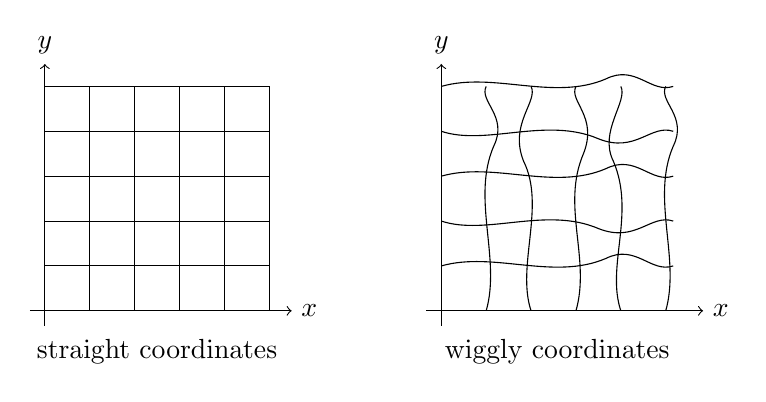
\begin{tikzpicture}[scale=0.95]
\begin{scope}
\draw[->] (-0.2,0) -- (3.3,0) node[right] {$x$};
\draw[->] (0,-0.2) -- (0,3.3) node[above] {$y$};
\foreach \u in {0.6,1.2,1.8,2.4,3.0}
{
\draw (\u,0) -- (\u,3.0);
\draw (0,\u) -- (3.0,\u);
}
\node at (1.5,-0.55) {straight coordinates};
\end{scope}
\begin{scope}[xshift=5.3cm]
\draw[->] (-0.2,0) -- (3.5,0) node[right] {$x$};
\draw[->] (0,-0.2) -- (0,3.3) node[above] {$y$};
\draw (0.6,0) .. controls (0.8,0.7) and (0.4,1.5) .. (0.7,2.2) .. controls (0.9,2.6) and (0.5,2.8) .. (0.6,3.0);
\draw (1.2,0) .. controls (1.0,0.6) and (1.4,1.4) .. (1.1,2.0) .. controls (0.9,2.5) and (1.3,2.8) .. (1.2,3.0);
\draw (1.8,0) .. controls (2.0,0.7) and (1.6,1.4) .. (1.9,2.1) .. controls (2.1,2.6) and (1.7,2.8) .. (1.8,3.0);
\draw (2.4,0) .. controls (2.2,0.6) and (2.6,1.3) .. (2.3,2.0) .. controls (2.1,2.4) and (2.5,2.8) .. (2.4,3.0);
\draw (3.0,0) .. controls (3.2,0.7) and (2.8,1.5) .. (3.1,2.2) .. controls (3.3,2.6) and (2.9,2.8) .. (3.0,3.0);
\draw (0,0.6) .. controls (0.7,0.8) and (1.5,0.4) .. (2.2,0.7) .. controls (2.6,0.9) and (2.8,0.5) .. (3.1,0.6);
\draw (0,1.2) .. controls (0.6,1.0) and (1.4,1.4) .. (2.1,1.1) .. controls (2.6,0.9) and (2.8,1.3) .. (3.1,1.2);
\draw (0,1.8) .. controls (0.7,2.0) and (1.5,1.6) .. (2.2,1.9) .. controls (2.6,2.1) and (2.8,1.7) .. (3.1,1.8);
\draw (0,2.4) .. controls (0.6,2.2) and (1.4,2.6) .. (2.1,2.3) .. controls (2.6,2.1) and (2.8,2.5) .. (3.1,2.4);
\draw (0,3.0) .. controls (0.7,3.2) and (1.5,2.8) .. (2.2,3.1) .. controls (2.6,3.3) and (2.8,2.9) .. (3.1,3.0);
\node at (1.55,-0.55) {wiggly coordinates};
\end{scope}
\end{tikzpicture}
\caption{A clean redraw of the lecture's point: the plane is still flat, but the coordinates themselves have acquired small ripples.}
\end{figure}

\section{Transverse-Traceless Waves and the Two Polarizations}

Once the spurious coordinate perturbations are cut away, the lecture turns to a real wave moving along the \(z\)-axis. A plane-wave dependence takes the form
\begin{align}
h_{\mu\nu}(t,z)\propto \sin k(z-t),
\end{align}
so the phase itself already tells us that the disturbance propagates with the speed of light.

The surviving physical components are transverse. The time components vanish, and so do the components parallel to the direction of propagation:
\begin{align}
h_{0\mu}=0,
\qquad
h_{z\mu}=0.
\end{align}
Thus only the transverse \(x\)-\(y\) plane remains. If we write \(i,j\in\{x,y\}\), the wave is described by
\begin{align}
h_{ij}(t,z)=h^{0}_{ij}\sin k(z-t),
\end{align}
with the symmetry
\begin{align}
h_{xy}=h_{yx}.
\end{align}
Einstein's equations then add one more restriction:
\begin{align}
h_{xx}+h_{yy}=0.
\end{align}
So the transverse perturbation is traceless.

\begin{figure}[t]
\centering

\includegraphics[width=0.84\textwidth]{lecture_10_figure_06.png}
\caption{Board evidence for the transverse-traceless wave moving along the \(z\)-axis, together with the traceless condition \(h_{xx}+h_{yy}=0\).}
\end{figure}

A convenient cleaned form of the final result is
\begin{align}
h_{ij}(t,z)
=
\begin{pmatrix}
h_{+} & h_{\times}\\
h_{\times} & -h_{+}
\end{pmatrix}
\sin k(z-t).
\end{align}
This makes the two independent polarization patterns completely explicit. In basis form,
\begin{align}
h^{(+)}_{ij}
=
\begin{pmatrix}
h_{+} & 0\\
0 & -h_{+}
\end{pmatrix},
\qquad
h^{(\times)}_{ij}
=
\begin{pmatrix}
0 & h_{\times}\\
h_{\times} & 0
\end{pmatrix}.
\end{align}
Every transverse-traceless gravitational wave traveling in the \(z\)-direction is a linear superposition of these two.

\begin{figure}[t]
\centering
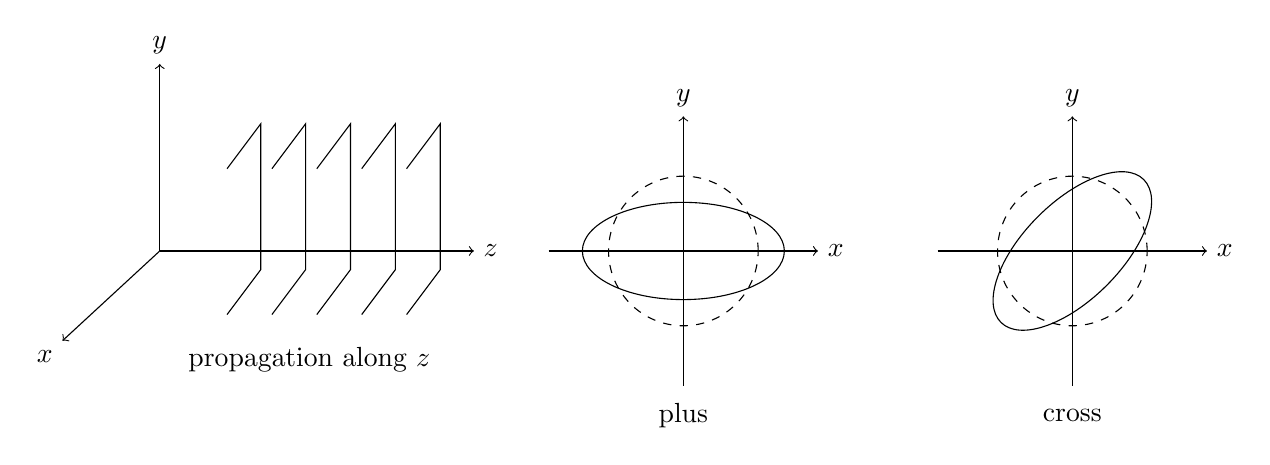
\begin{tikzpicture}[scale=0.95]
\begin{scope}
\draw[->] (0,0) -- (4.2,0) node[right] {$z$};
\draw[->] (0,0) -- (0,2.5) node[above] {$y$};
\draw[->] (0,0) -- (-1.3,-1.2) node[below left] {$x$};
\foreach \s in {0.9,1.5,2.1,2.7,3.3}
{
\draw (\s,1.1) -- (\s+0.45,1.7) -- (\s+0.45,-0.25) -- (\s,-0.85);
}
\node at (2.0,-1.45) {propagation along \(z\)};
\end{scope}
\begin{scope}[xshift=7.0cm]
\draw[->] (-1.8,0) -- (1.8,0) node[right] {$x$};
\draw[->] (0,-1.8) -- (0,1.8) node[above] {$y$};
\draw[dashed] (0,0) circle (1.0);
\draw (0,0) ellipse (1.35 and 0.65);
\node at (0,-2.2) {plus};
\end{scope}
\begin{scope}[xshift=12.2cm]
\draw[->] (-1.8,0) -- (1.8,0) node[right] {$x$};
\draw[->] (0,-1.8) -- (0,1.8) node[above] {$y$};
\draw[dashed] (0,0) circle (1.0);
\draw[rotate=45] (0,0) ellipse (1.35 and 0.65);
\node at (0,-2.2) {cross};
\end{scope}
\end{tikzpicture}
\caption{A clean redraw of the lecture's geometry: a wave propagating along the \(z\)-axis, and the two independent transverse deformations.}
\end{figure}

\section{What the Wave Does to Matter}

This is the point at which the lecture shifts from algebra to geometry. Fix a value of \(z\) and \(t\), and look at the two-dimensional transverse slice. The induced metric in that plane is
\begin{align}
ds_{\perp}^{2}
=
(1+h_{xx})\,dx^{2}
+
2h_{xy}\,dx\,dy
+
(1+h_{yy})\,dy^{2}.
\end{align}
For a pure plus mode one has \(h_{xy}=0\) and \(h_{yy}=-h_{xx}\), so
\begin{align}
g_{xx}=1+h_{xx},
\qquad
g_{yy}=1-h_{xx}.
\end{align}
If \(h_{xx}>0\), proper distances along the \(x\)-direction are slightly enlarged, while those along the \(y\)-direction are slightly reduced. Half a cycle later the sine changes sign, and the roles of \(x\) and \(y\) reverse. A square piece of matter is therefore alternately stretched horizontally and compressed vertically, then compressed horizontally and stretched vertically.

For the cross mode the same thing happens after a rotation by \(45^\circ\). There is no new physics there, only a new orientation of the same transverse squeeze-and-stretch pattern. This is why the lecture treats the two polarizations as a basis: any real wave is built from them by superposition.

\subsection{Question \& Answer}

Is the meter stick itself changing, or should we really think instead about two test masses?

The lecture's answer is subtle and worth preserving. A real object is held together by internal forces. A steel rod and a wooden rod will not respond in exactly the same way to the same passing gravitational wave. So one should not imagine an absolutely rigid standard ruler that simply rides through the wave untouched. The passing wave carries real curvature and produces tidal stresses. A strain gauge can register those stresses; two separated test masses can register the relative motion. Either way, what is being measured is not a coordinate trick but a genuine physical response to curvature.

This is also why the lecture insists that an oscillating wave is different from a merely static deformation. The oscillation creates real alternating stresses and strains. The wave is not just a relabeling of space; it is a moving pattern of curvature.

\subsection{Question \& Answer}

If all components with a time index vanish, does that mean there is no curvature in the time direction?

No. The vanishing of \(h_{0\mu}\) is a statement about the allowed physical components of the metric perturbation in the transverse-traceless description. Curvature, however, is built from derivatives of those surviving components. In particular,
\begin{align}
\partial_t h_{ij}\neq 0,
\qquad
R_{\mu\nu\rho\sigma}\sim \partial\partial h.
\end{align}
So even though the perturbation carries only transverse spatial indices, its time dependence still contributes to the curvature tensor. The lecture compares this to electromagnetism: a wave moving along the \(z\)-axis may be described entirely by transverse field components and yet still be fully dynamical in time.

\section{Sources, Detection, and Another Way of Thinking}

By now the gravitational wave is no longer an abstract perturbation. It is a traveling curvature disturbance with a definite polarization structure and measurable tidal effect. The lecture then widens the aperture.

Accelerating masses generate gravitational waves just as accelerating charges generate electromagnetic radiation. A binary pulsar is the lecture's preferred example: two compact masses orbiting one another, producing strong gravitational dynamics near the source and weak radiation far away. Close to the source the linear approximation is poor. Far from it, the field dilutes, \(h_{\mu\nu}\) becomes small, and the weak-field analysis becomes reliable.

The lecture also stresses how tiny the far-zone effect is. The strain expected from distant astrophysical sources is extremely small, of order \(10^{-21}\) in the lecture's discussion. That is why detection requires either resonance or interferometric precision. A detector must provide a system that can be driven by the passing wave. In that sense the lecture treats LIGO not as a mystery device but as a refined descendant of the same physical idea: the wave produces a differential transverse effect, and one measures that differential effect as sensitively as possible.

Finally, there is the indirect evidence from the binary pulsar. Radiation carries energy away. If a binary system emits gravitational waves, its orbital motion must drift accordingly. The lecture emphasizes that the observed timing change of the system matches precisely what one expects from gravitational radiation. That is the historical payoff of the weak-wave story as it was told in the lecture: the waves are real, even when they are incredibly weak.

\subsection{Another Way of Thinking: The Action Principle}

With a little time left, the lecture changes register. Instead of asking directly for the field equations, it asks what invariant action could produce them.

The setting is field theory. A field history assigns values of the field at every point of spacetime. Not every imaginable field history solves the equations of motion. The actual histories are the ones that make the action stationary, subject to the boundary data.

Before writing the gravitational action, the lecture first reconstructs the invariant volume element. In two spatial dimensions, if the metric is diagonal,
\begin{align}
ds^{2}=g_{xx}\,dx^{2}+g_{yy}\,dy^{2},
\end{align}
then the proper lengths of the sides of a small rectangle are \(\sqrt{g_{xx}}\,dx\) and \(\sqrt{g_{yy}}\,dy\). Its area is therefore
\begin{align}
dA=\sqrt{g_{xx}}\,dx\,\sqrt{g_{yy}}\,dy.
\end{align}
Once off-diagonal terms are allowed, the product \(g_{xx}g_{yy}\) is replaced by the determinant, so in general
\begin{align}
dA=\sqrt{\det g}\,dx\,dy.
\end{align}
In three-dimensional space this becomes the volume element
\begin{align}
dV=\sqrt{\det g}\,dx\,dy\,dz.
\end{align}
And in spacetime the same idea leads to the invariant four-volume element
\begin{align}
dV_{4}=\sqrt{|g|}\,d^{4}x,
\end{align}
where \(g=\det(g_{\mu\nu})\).

Now if \(S(x)\) is any scalar field, then
\begin{align}
\int d^{4}x\,\sqrt{|g|}\,S(x)
\end{align}
is invariant under coordinate changes. This is exactly the kind of object an action in general relativity ought to be, because the laws of physics should not depend on the coordinate system.

For pure gravity in vacuum, the natural scalar built from the metric is the scalar curvature \(R\). Thus the gravitational action is
\begin{align}
S_{\mathrm{grav}}=\int d^{4}x\,\sqrt{|g|}\,R.
\end{align}
One may also add a constant scalar, the cosmological constant:
\begin{align}
S_{\Lambda}=\Lambda\int d^{4}x\,\sqrt{|g|}.
\end{align}
The lecture is careful here: the weak-wave equations discussed earlier were the vacuum equations without the cosmological constant, so the wave analysis should not be muddled with that extra term.

The conceptual claim is then simple even if the variation is not. One varies the metric, treats the action as a functional of \(g_{\mu\nu}\), and imposes stationarity. The resulting Euler-Lagrange equations are Einstein's equations. Matter and other fields enter by adding further invariant scalar densities to the action. In the electromagnetic case, for example, one builds the matter part from the field tensor \(F_{\mu\nu}\) and combines it with the same invariant measure \(\sqrt{|g|}\,d^{4}x\).

The lecture ends this way for a reason. The brute-force computation is ugly; the principle behind it is clean.

\section{Summary}

The story of weak gravitational waves is the story of a controlled approximation about empty flat spacetime. We linearize \(g_{\mu\nu}=\eta_{\mu\nu}+h_{\mu\nu}\), keep only first-order terms, recognize the wave-equation structure, and then face the decisive fact that not every small \(h_{\mu\nu}\) is physical. After the coordinate artifacts are removed, a wave moving along the \(z\)-axis carries only two transverse-traceless polarizations. Those polarizations are not bookkeeping devices: they describe real tidal curvature, real strain, and real energy transport. The lecture then closes by stepping back once more. The same Einstein equations that govern these weak waves may be viewed as the stationary-point condition of the Einstein-Hilbert action, where invariant spacetime volume and scalar curvature are the essential ingredients.